\documentclass[11pt,a4paper]{article}

\usepackage[utf8]{inputenc}
\usepackage{geometry}
\geometry{a4paper, margin=2.5cm}
\usepackage{graphicx}
\usepackage{booktabs}
\usepackage{hyperref}
\usepackage{float}
\usepackage{enumitem}
\usepackage{parskip}

\title{\textbf{Kafka Fraud Sentinel} \\ \large Real-Time Fraud Detection System}
\author{Giacomo Comitani - 85673A}
\date{August 2026}

\begin{document}
\maketitle
\thispagestyle{empty}

\begin{center}
    \large \textit{Project Report -- Cloud Computing Technologies}\\[0.2em]
    \normalsize University of Milan (UNIMI), Academic Year 2025/2026
\end{center}

\begin{abstract}
This report presents Kafka Fraud Sentinel, a distributed, real-time fraud detection system built on Apache Kafka. Developed for the Cloud Computing Technologies course, the project simulates a Security Operations Center (SOC) capable of ingesting high volumes of financial transactions and instantly identifying anomalous patterns, such as velocity and amount frauds. The architecture is entirely containerized using Docker and leverages a 3-node KRaft cluster to ensure high availability and fault tolerance. Strict security boundaries are enforced through mutual TLS (mTLS) authentication and fine-grained Access Control Lists (ACLs). Verified alerts are persisted in MongoDB, streamed to a live web dashboard via WebSockets, and forwarded to administrators via a Telegram bot.
\end{abstract}
\newpage

\section{Project Overview}
For this Cloud Computing project was developed a distributed system that analyzes financial transactions in real time to catch potential frauds. 

Instead of building a classic REST API where services talk directly to each other, an event-driven approach based on Apache Kafka was chosen. In a real-world bank, thousands of transactions happen every second. If the fraud detection engine experiences a temporary outage, the system cannot afford to lose the transactions or block users from making payments. Kafka acts as a durable buffer: producers simply send transactions to a topic, and consumers process them at their own pace.

The main goals of the project are:
\begin{itemize}
    \item Real-time data processing using Python.
    \item A secure environment using SSL certificates (mTLS) and ACLs, ensuring no unauthorized access.
    \item High availability, ensuring the system survives if a server crashes.
\end{itemize}

\section{Infrastructure Setup}
The entire infrastructure is containerized using Docker Compose. The core is a Kafka cluster composed of 3 brokers running in KRaft mode, meaning there is no ZooKeeper dependency. A MongoDB container is also included to save the alerts, along with AKHQ to monitor the cluster via a web interface.

\subsection{Topics and Partitioning}
During the Kafka setup, two separate topics were created. This separation is a key design choice:
\begin{itemize}
    \item \texttt{transactions}: this is the main topic where all the generated transactions arrive. It handles high traffic.
    \item \texttt{fraud-alerts}: this topic only receives the suspicious transactions. It has very low traffic.
\end{itemize}

Both topics are configured with 3 partitions and a replication factor of 3. The \texttt{min.insync.replicas} parameter is set to 2. This setup guarantees that every message is copied on all three brokers, and a write is considered successful only if at least two brokers save it on disk.

When producing messages to the \texttt{transactions} topic, the \texttt{user\_id} is used as the Kafka key. This is fundamental for the fraud detection logic. Kafka guarantees that messages with the same key always go to the same partition. This means the consumer reads the transactions of a specific user in the exact chronological order they were made, which is mandatory to detect velocity frauds accurately.

\section{Application Components}
The codebase is divided into distinct Python microservices. Figure \ref{fig:arch} shows how they interact.

\begin{figure}[H]
    \centering
    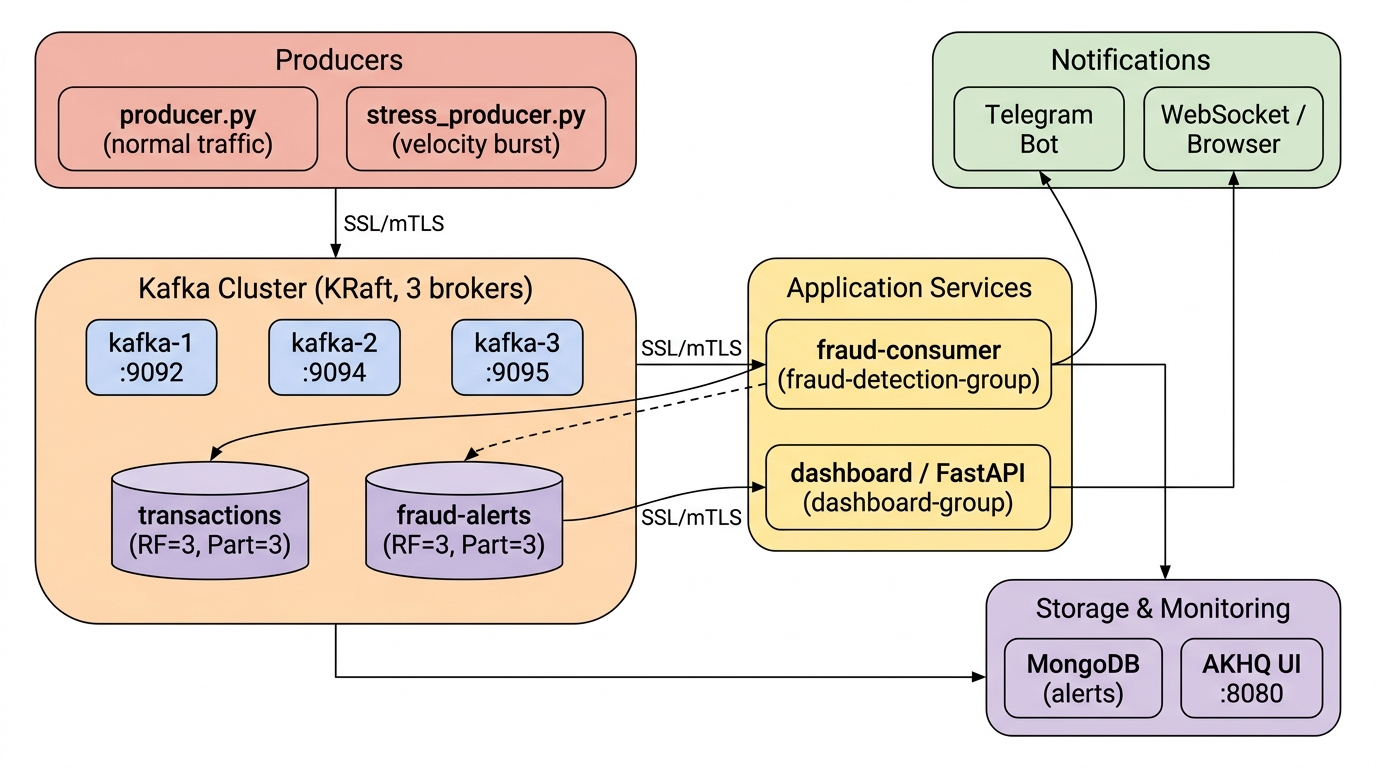
\includegraphics[width=0.92\textwidth]{images/architecture_diagram.jpg}
    \caption{Architecture of the system.}
    \label{fig:arch}
\end{figure}

\subsection{Data Generation (Producers)}
To test the system, a \texttt{producer.py} script continuously generates mock transactions for 100 different users. It is programmed to mix normal traffic with fraudulent behavior:
\begin{itemize}
    \item About 30\% of the transactions have a very high amount (above 1000 EUR).
    \item About 15\% of the time, the producer picks a random user and sends a "burst" of 4 to 6 transactions in less than a second.
\end{itemize}

A \texttt{stress\_producer.py} script is also provided, which can be triggered on-demand from the web dashboard. It targets a single user (\texttt{user\_101}) with 15 rapid transactions to show how the system reacts to sudden spikes.

\subsection{Fraud Detection Engine (Consumer)}
The \texttt{consumer.py} script is the analytical core of the project. It belongs to the \texttt{fraud-detection-group} and continuously reads from the \texttt{transactions} topic. 

For every message, it runs two checks:
\begin{enumerate}
    \item \textbf{Amount Fraud}: A simple stateless check. If the transaction amount is strictly greater than 5000 EUR, it triggers an alert.
    \item \textbf{Velocity Fraud}: A stateful check. A sliding window is implemented in Python using a dictionary. The consumer keeps track of the timestamps of the recent transactions for every user. If a user makes more than 3 transactions in a 10-second window, it is flagged as a velocity fraud.
\end{enumerate}

When a fraud is found, the consumer performs three actions: it saves the full alert details into MongoDB, it produces a message into the \texttt{fraud-alerts} topic, and it sends a push notification to an administrator via Telegram.

\begin{figure}[H]
    \centering
    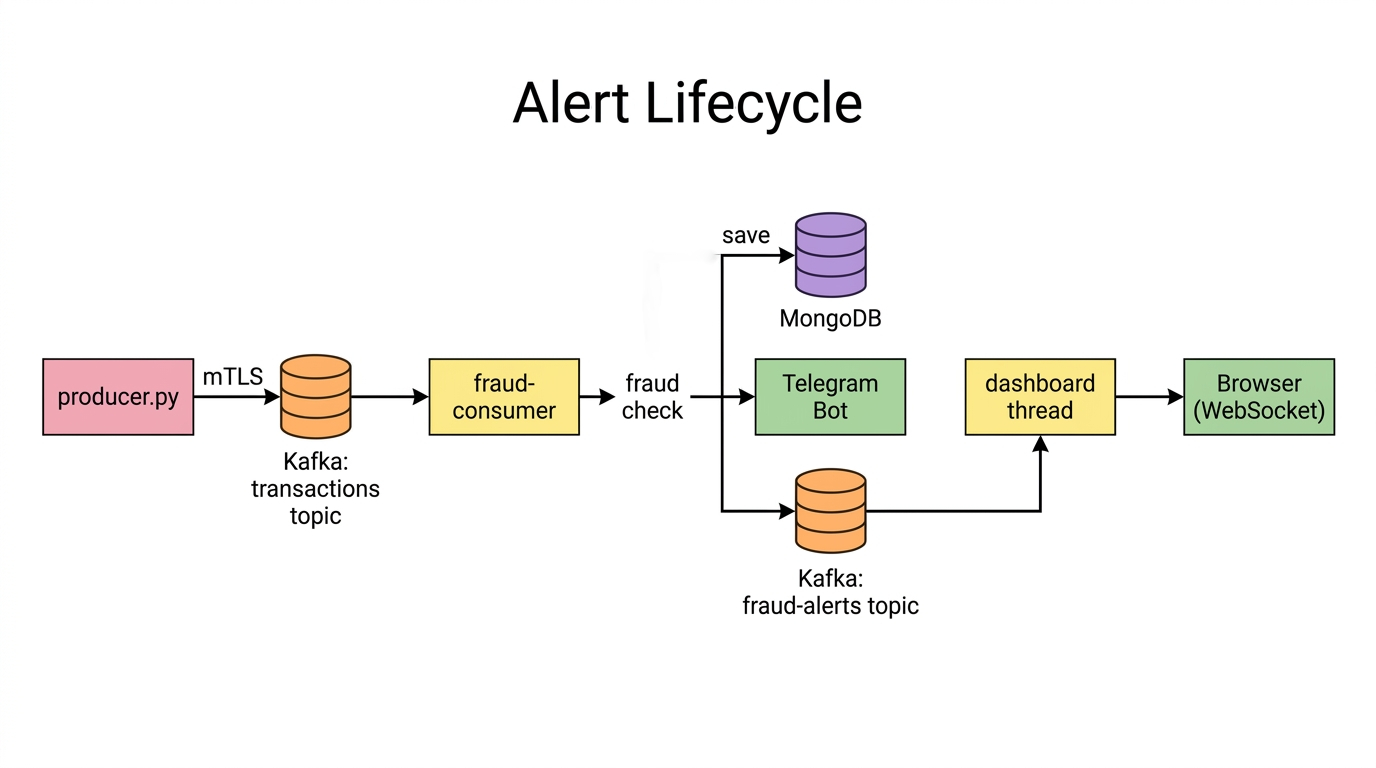
\includegraphics[width=0.95\textwidth]{images/alert_lifecycle_diagram.jpg}
    \caption{Alert lifecycle.}
    \label{fig:lifecycle}
\end{figure}

\subsection{Real-Time Dashboard}
To provide a visual representation of the incoming frauds, a lightweight web server is built using FastAPI. The server runs a background thread connected to Kafka (in its own \texttt{dashboard-group}), listening to the \texttt{fraud-alerts} topic.

When an alert arrives, the dashboard pushes it instantly to the web browser using WebSockets. The web page also has buttons to manually trigger the producers and test the system. Since it also connects to MongoDB, refreshing the page does not clear the past alerts.

\begin{figure}[H]
    \centering
    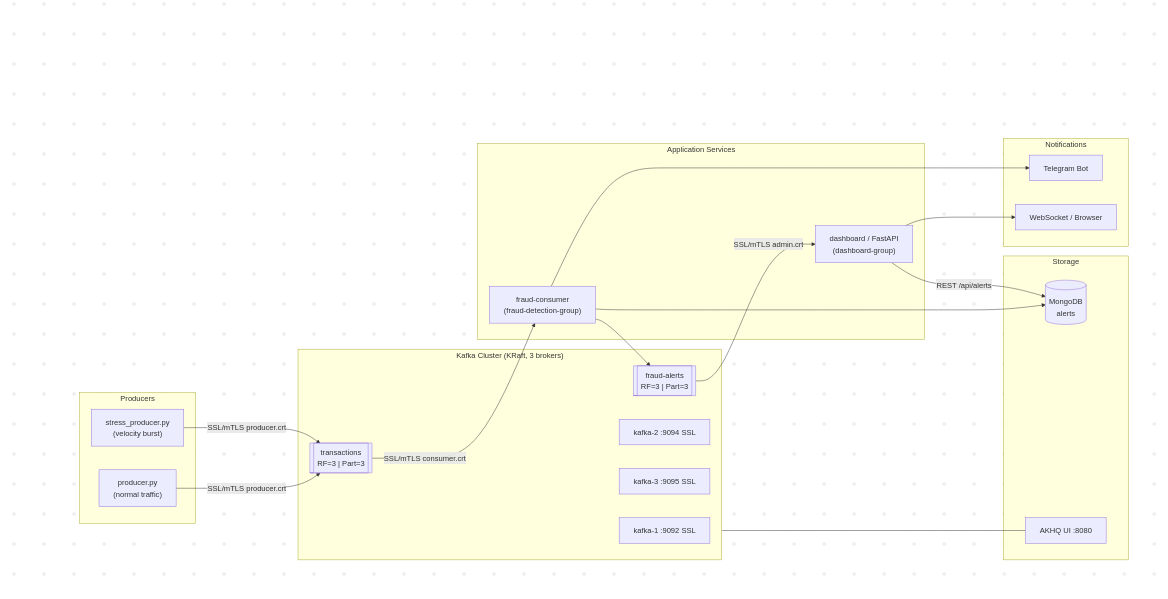
\includegraphics[width=0.88\textwidth]{images/kafka_dashboard.png}
    \caption{The web dashboard showing real-time alerts.}
    \label{fig:dashboard}
\end{figure}

\section{Security Implementation}
Implementing security is a core requirement of the project. No microservice is allowed to connect to Kafka without proving its identity.

\subsection{Mutual TLS (mTLS)}
Instead of using simple passwords, mTLS is used. A bash script acts as a custom Certificate Authority (CA). The script generates certificates for the 3 Kafka brokers and for the 3 roles of the applications: \texttt{producer}, \texttt{consumer}, and \texttt{admin} (for the dashboard).

When a Python script connects to Kafka, it presents its certificate. If the certificate is missing or invalid, Kafka drops the connection immediately during the TLS handshake. This ensures all traffic is encrypted and only authorized scripts can connect.

\subsection{Access Control Lists (ACLs)}
After authenticating, a script must be authorized. The Kafka ACLs are configured so that every certificate has only the strict permissions it needs. For example:
\begin{itemize}
    \item The producer can write to \texttt{transactions}, but cannot read from it.
    \item The fraud-consumer can read from \texttt{transactions} and write to \texttt{fraud-alerts}.
    \item The dashboard admin can only read from \texttt{fraud-alerts}.
\end{itemize}

An interesting issue with KRaft was encountered during development. Initially, the \texttt{ANONYMOUS} user was removed from the super-users list, but the brokers crashed at startup. It was discovered that the internal KRaft controllers communicate using the ANONYMOUS principal before the ACL engine is fully loaded. It had to be restored, but the risk is minimal because the internal ports are not exposed outside the Docker network.

\section{Testing and Demos}
Several scenarios are provided to demonstrate that the system works as expected under adverse conditions.

\subsection{Broker Crash Survival}
A bash script (\texttt{demo-broker-failure.sh}) violently stops one of the Kafka brokers (\texttt{kafka-2}) while the producer is running. Because of the configuration (\texttt{acks=all}, \texttt{min.insync.replicas=2}), the producer does not crash and no data is lost. The system simply continues working with the remaining two brokers. When \texttt{kafka-2} is restarted, it syncs back up automatically.

\subsection{Security Tests}
Two "attacker" scripts are included to test the security boundaries. One tries to connect in plaintext, and the other tries to connect with SSL but without the client certificate. In both cases, Kafka rejects the connection and the dashboard does not show any fake transactions.

\subsection{Offset Recovery}
A \texttt{recovery\_demo.py} script is included to show how consumer offsets work. If a consumer crashes while reading, Kafka remembers exactly where it stopped. When the script is restarted, it resumes processing from the exact same point without duplicating or skipping messages.

\subsection{Telegram Notifications}
To ensure that system administrators are immediately informed of suspicious activities, a Telegram bot integration is implemented. If the bot credentials are provided in the environment variables, the fraud-consumer automatically dispatches a Markdown-formatted alert message to the designated chat. This provides a mobile-friendly monitoring solution alongside the web dashboard.

\begin{figure}[H]
    \centering
    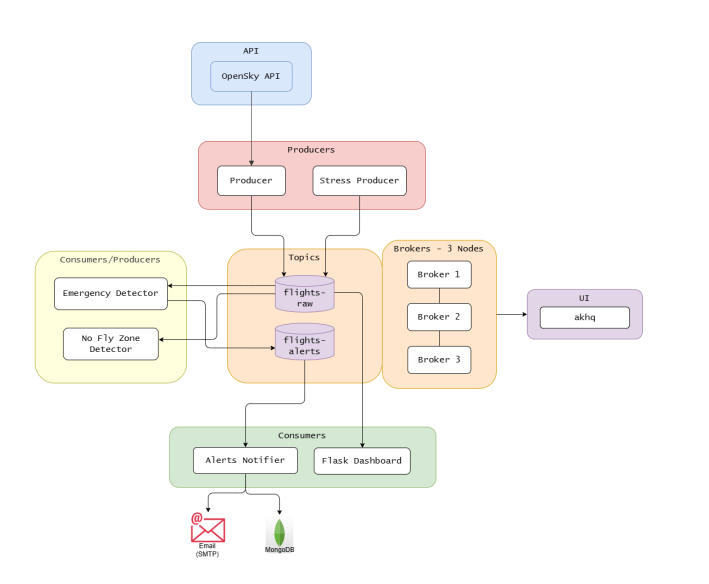
\includegraphics[width=0.50\textwidth]{images/mockup.png}
    \caption{Telegram alerts delivered directly to the administrator's phone.}
    \label{fig:telegram}
\end{figure}

\section{Limitations and Future Improvements}
This project serves as a solid prototype, but for a real production environment, a few architectural changes would be necessary:
\begin{itemize}
    \item \textbf{Externalize State}: The velocity fraud counter is kept in a Python dictionary. If the \texttt{consumer.py} crashes, the memory is wiped and the current 10-second window is lost. This state should be moved to a Redis database to make it persistent across restarts.
    \item \textbf{Dynamic Rules}: Currently, the 5000 EUR limit is hardcoded. It would be better to fetch this threshold from a database or use a machine learning model to detect anomalies based on a user's past behavior.
    \item \textbf{Exactly-Once Semantics}: If the consumer writes to MongoDB and crashes right before sending the message to the \texttt{fraud-alerts} topic, the system might process that transaction twice when it restarts. Implementing exactly-once semantics would solve this edge case.
\end{itemize}

\section{Conclusion}
The development of "Kafka Fraud Sentinel" demonstrates exactly why standard databases or REST APIs are not suited for streaming events. Setting up the Kafka cluster with KRaft and writing the producer/consumer logic is straightforward, but configuring mTLS and ACLs correctly is challenging and highly instructive. Seeing the system survive a live broker crash without dropping a single transaction effectively proves the resilience of the architecture.

\end{document}
